%%%%%%%%%%%%%%%%%%%%%%%%%%%%%%%%%%%%%%%%%%%%%%%%%%%%%%%%%%%%%%%%%%%%%%%%%%%%%%%%%%%%%%
% Modelo de relatório de Disciplina de MLP a partir da
% classe latex iiufrgs disponivel em http://github.com/schnorr/iiufrgs
%%%%%%%%%%%%%%%%%%%%%%%%%%%%%%%%%%%%%%%%%%%%%%%%%%%%%%%%%%%%%%%%%%%%%%%%%%%%%%%%%%%%%%

% Ignore o comentario acima e imagine que exista um modelo de relatorio de CCI em algum lugar

%%%%%%%%%%%%%%%%%%%%%%%%%%%%%%%%%%%%%%%%%%%%%%%%%%%%%%%%%%%%%%%%%%%%%%%%%%%%%%%%%%%%%%
% Definição do tipo / classe de documento e estilo usado
%%%%%%%%%%%%%%%%%%%%%%%%%%%%%%%%%%%%%%%%%%%%%%%%%%%%%%%%%%%%%%%%%%%%%%%%%%%%%%%%%%%%%%
%
\documentclass{iiufrgs}

%%%%%%%%%%%%%%%%%%%%%%%%%%%%%%%%%%%%%%%%%%%%%%%%%%%%%%%%%%%%%%%%%%%%%%%%%%%%%%%%%%%%%%
% Importação de pacotes
%%%%%%%%%%%%%%%%%%%%%%%%%%%%%%%%%%%%%%%%%%%%%%%%%%%%%%%%%%%%%%%%%%%%%%%%%%%%%%%%%%%%%%
% (a A seguir podem ser importados os pacotes necessários para o documento, de acordo 
% com a necessidade)
%
\usepackage[brazilian]{babel}	    % para texto escrito em pt-br
\usepackage[utf8]{inputenc}         % pacote para acentuação
\usepackage{graphicx}         	    % pacote para importar figuras
\usepackage[T1]{fontenc}            % pacote para conj. de caracteres correto
\usepackage{times}                  % pacote para usar fonte Adobe Times
\usepackage{enumerate}              % para lista de itens com letras
\usepackage{breakcites}
\usepackage{tikz}
\usepackage[oldvoltagedirection]{circuitikzgit}
\usepackage{caption}
\usepackage{siunitx}
\usepackage{placeins}
\usepackage{titlesec}
\usepackage{enumitem}
\usepackage{titletoc}               
%\usepackage{listings}			    % para listagens de código-fonte
\usepackage{mathptmx}               % p/ usar fonte Adobe Times nas formulas matematicas
\usepackage{url}                    % para formatar URLs
%\usepackage{color}				    % para imagens e outras coisas coloridas
\usepackage{fixltx2e}              % para subscript
%\usepackage{amsmath}               % para \epsilon e matemática
%\usepackage{amsfonts}
%\usepackage{setspace}			    % para mudar espaçamento dos parágrafos
%\usepackage[table,xcdraw]{xcolor}  % para tabelas coloridas
%\usepackage{longtable}             % para tabelas compridas (mais de uma página)
%\usepackage{float}
%\usepackage{booktabs}
\usepackage{tabularx}
%\usepackage{hyperref}

\usepackage[alf,abnt-emphasize=bf]{abntex2cite}	% pacote para usar citações abnt

%%%%%%%%%%%%%%%%%%%%%%%%%%%%%%%%%%%%%%%%%%%%%%%%%%%%%%%%%%%%%%%%%%%%%%%%%%%%%%%%%%%%%%
% Macros, ajustes e definições
%%%%%%%%%%%%%%%%%%%%%%%%%%%%%%%%%%%%%%%%%%%%%%%%%%%%%%%%%%%%%%%%%%%%%%%%%%%%%%%%%%%%%%
%

% define estilo de parágrafo para citação longa direta:
\newenvironment{citacao}{
    %\singlespacing
    %\footnotesize
    \small
    \begin{list}{}{
        \setlength{\leftmargin}{4.0cm}
        \setstretch{1}
        \setlength{\topsep}{1.2cm}
        \setlength{\listparindent}{\parindent}
    }
    \item[]}{\end{list}
}

% adiciona a fonte em figuras e tabelas
\newcommand{\fonte}[1]{\\Fonte: {#1}}

\newcommand{\virtuoso}{\textit{Virtuoso}}

\newcommand{\titlepagespecificinfo}{Relatório apresentado como requisito parcial para a obtenção de conceito na Disciplina de Concepção de Circuitos Integrados.}
% \def\@cipspecificinfo{Concepção de Circuitos Integrados}


% Ative o seguinte caso alguma nota de rodapé fique muito longa e quebre entre múltiplas
% páginas
%\interfootnotelinepenalty=10000

%%%%%%%%%%%%%%%%%%%%%%%%%%%%%%%%%%%%%%%%%%%%%%%%%%%%%%%%%%%%%%%%%%%%%%%%%%%%%%%%%%%%%%
% Informações gerais                                   
%%%%%%%%%%%%%%%%%%%%%%%%%%%%%%%%%%%%%%%%%%%%%%%%%%%%%%%%%%%%%%%%%%%%%%%%%%%%%%%%%%%%%%

% título
\title{RELATÓRIO 1} 

% autor
%\author{Autores(s)}{Aluno(s)} % {sobrenome}{nome}
\author{Silva}{Henrique Corrêa Pereira da}

% Professor orientador da disciplina
\advisor[Prof.~Dr.]{Augusto Da Luz Reis}{Ricardo}

% Nome do(s) curso(s):
\course{Curso de Graduação em Ciência da Computação}

% local da realização do trabalho 
\location{Porto Alegre}{RS} 

% data da entrega do trabalho (mês e ano)
\date{4}{2018}


% Palavras chave
\keyword{CCI}
\keyword{Virtuoso}
\keyword{Inversor}
\keyword{Relatório}


%%%%%%%%%%%%%%%%%%%%%%%%%%%%%%%%%%%%%%%%%%%%%%%%%%%%%%%%%%%%%%%%%%%%%%%%%%%%%%%%%%%%%%
% Início do documento e elementos pré-textuais
%%%%%%%%%%%%%%%%%%%%%%%%%%%%%%%%%%%%%%%%%%%%%%%%%%%%%%%%%%%%%%%%%%%%%%%%%%%%%%%%%%%%%%

% Declara início do documento
\begin{document}

% inclui folha de rosto 
\maketitle

\selectlanguage{brazilian}

% Sumario
\tableofcontents



%%%%%%%%%%%%%%%%%%%%%%%%%%%%%%%%%%%%%%%%%%%%%%%%%%%%%%%%%%%%%%%%%%%%%%%%%%%%%%%%%%%%%
% Aqui comeca o texto propriamente dito
%%%%%%%%%%%%%%%%%%%%%%%%%%%%%%%%%%%%%%%%%%%%%%%%%%%%%%%%%%%%%%%%%%%%%%%%%%%%%%%%%%%%%

%espaçamento entre parágrafos
%\setlength{\parskip}{6 pt}

\selectlanguage{brazilian}

%%%%%%%%%%%%%%%%%%%%%%%%%%%%%%%%%%%%%%%%%%%%%%%%%%%%%%%%%%%%%%%%%%%%%%%%%%%%%%%%%%%%%
% Introdução
%

%Este capítulo tem o objetivo de descrever os detalhes necessários à correta formatação do documento. As informações aqui apresentadas devem ser suficientes para formatar corretamente o documento no ambiente \LaTeX.

%Os \textbf{Capítulos} são sempre iniciados com o comando \texttt{\char'134chapter}, que coloca-os em uma nova folha, em letras maiúsculas, numerados e  alinhados à esquerda. Para os \textbf{capítulos não-numerados} (Listas, Resumo, Abstract, Referências, etc.), o título é centralizado na linha Para tanto, usar o comando \texttt{\char'134chapter*}. Para ambos, são deixados 90 pt de espaçamento anterior (ou seja, distância da margem superior) e 42 pt de espaçamento posterior (espaço até o início do texto ou primeira subdivisão). 

%Todos os \textbf{demais parágrafos de texto} são escritos em espaçamento simples, com observância de 6 pt de espaçamento em relação ao parágrafo seguinte. O estilo atual já considera essas retrições. 


%As demais subdivisões do texto (seções, subseções, etc.) são formatadas com o título alinhado sempre à esquerda, precedido da respectiva numeração. Para tanto, no \LaTeX, você deve utilizar os comandos \texttt{\char'134section},  \texttt{\char'134subsection} e  \texttt{\char'134subsubsection}.

%São permitidas subdivisões até o 5º nível (onde o capítulo é o 1º. nível), porém no sumário inclui-se somente os títulos até o nível 3\footnote{O formato adotado pela ABNT prevê apenas três níveis (capítulo, seção e subseção).}. Assim, \texttt{\char'134subsubsection} não é aconselhado. 


%%%%%%%%%%%%%%%%%%%%%%%%%%%%%%%%%%%%%%%%%%%%%%%%%%%%%%%%%%%%%%%%%%%%%%%%%%%%%%%%%%%%%
% Visao Geral
%

\chapter{Introdução}\label{intro}

Neste relatório, construiremos leiautes e esquemáticos de quatro especificações de inversor 
utilizando diferentes tamanhos de transistor e compararemos sua performance utilizando as 
seguintes métricas:

\begin{enumerate}[leftmargin=3em, noitemsep] % [label={--}]
    \setlength{\itemindent}{1em}
    \item T\textsubscript{lh}: tempo de subida do sinal;
    \item T\textsubscript{hl}: tempo de descida do sinal;
    \item Tp\textsubscript{lh}: tempo de propagação \textit{low-high}; 
    \item Tp\textsubscript{hl}: tempo de propagação \textit{high-low}; 
    \item Tp\textsubscript{médio}: tempo de propagação médio; 
    \item P\textsubscript{média}: potência média do circuito; 
    \item P\textsubscript{RMS}: potência \textit{RMS} do circuito.
\end{enumerate}

Além disso, será feita a análise \textit{Layout versus Schematic} para cada inversor a fim de 
verificar a funcionalidade do leiaute contra o esquemático. Mais detalhes sobre a implementação 
dos transistores e do circuito no Capítulo \ref{proposta}. \

\begin{figure}[htb]
    \centering
    \caption{Circuito a ser projetado.}
    \label{fig:circuito}
    \begin{circuitikz}
        \node (source) at (0, 2) {};
        \node [ground] (gnd1) at (0, 0) {};
        \node [ground] (gnd2) at (6, 0) {};
        \node [american not port] (not1) at (1.5, 2) {};
        \node [american not port] (not2) at (3, 2) {};
        \node [american not port] (not3) at (4.5, 2) {};
        \node (out) at (6, 2) {};
        \draw (gnd1) to[vsourcesquare, v=$3.3 V$] (source);
        \draw (source) to[short] (not1.in);
        \draw (not1.out) |- (not2.in);
        \draw (not2.out) |- (not3.in);
        \draw (not3.out) to[short] (out);
        \draw (gnd2) to[pC, l_=$50fF$] (out);
        \node at (0, 3.5) {};
        \node at (1.5, 3) {$INV_1$};
        \node at (1.5, 1) {$Impl._1$};
        \node at (3, 3) {$INV_2$};
        \node at (4.5, 3) {$INV_1$};
        \node at (4.5, 1) {$Impl._1$};
    \end{circuitikz}
\end{figure}

\chapter{Proposta}\label{proposta}
A proposta do relatório é realizar o redimensionamento do INV\textsubscript{2}, variando os valores de W\textsubscript{p} e de W\textsubscript{n} conforme a Tabela \ref{tab:imp}.
Além disso, o circuito também deverá seguir as seguintes especificações:

\begin{itemize}[noitemsep]
    \setlength{\itemindent}{1em}
    \item VDD = \SI{3.3}{\V};
    \item $1/f$ = \SI{10}{\ns};
    \item T\textsubscript{rise} = \SI{200}{\ps};
    \item T\textsubscript{fall} = \SI{200}{\ps};
    \item P\textsubscript{width} = \SI{5}{\ns}.
\end{itemize}

Criados os novos leiautes, é obrigatório tanto o teste individual de cada um utilizando as ferramentas \textit{DRC} e \textit{LVS} quanto a extração das capacitâncias parasitas de cada implementação.
Dado este passo completo, a última etapa consiste em criar um novo \textit{cellview} para cada versão do circuito da Figura \ref{fig:circuito}.

\begin{table}[ht]
    \centering
    \caption{Dimensões em cada implementação.}
    \label{tab:imp}
    \begin{tabular}{l c c}
        \hline
        Implementação
        & W\textsubscript{p}
        & W\textsubscript{n} \\ \hline
        \#1 & \SI{1.5}{\um}     & \SI{1.0}{\um}     \\ 
        \#2 & \SI{1.0}{\um}     & \SI{1.0}{\um}     \\ 
        \#3 & \SI{10.5}{\um}    & \SI{7.0}{\um}     \\ 
        \#4 & \SI{7.0}{\um}     & \SI{10.5}{\um}    \\ \hline
    \end{tabular}
\end{table}

\chapter{Análise}\label{analise}
Neste capítulo abordaremos cada implementação do inversor e, no Capítulo \ref{resultados} analisaremos os resultados e faremos algumas observações sobre o circuito simulado.

\section{Inversores}
A Figura \ref{fig:inversor} mostra o esquemático do inversor estático CMOS que implementaremos. Quando o V\textsubscript{in} é alto e igual à V\textsubscript{DD}, o transistor NMOS está ativo, enquanto o PMOS está desativado.\

Isso garante que, para qualquer dado momento em condições operacionais, não exista um caminho direto da fonte para o dreno. Essa ausência de fluxo de corrente define que a porta lógica não gaste energia passivamente \footnote{salvo possíveis vazamentos.}.\

A observação anterior, embora pareça óbvia, é de crucial importância, pois, utilizando uma implementação com tecnologia NMOS pura, a rede pull-up tem potência estática não trivial, o que resulta num limite máximo de portas que podem ser implementadas num só \textit{die} \cite{Rabaey1996Circuits}.\

\begin{figure}[htb]
    \centering
    \caption{Esquemático de um inversor CMOS.}
    \label{fig:inversor}
    \begin{circuitikz}
        \node [pmos] (pmos) at (2, 3) {};
        \node [nmos] (nmos) at (2, 1) {};
        \draw (pmos.S) to[short, -*] node[above] {$V_{DD}$} ++(0, 0.5);
        \draw (pmos.D) -- (nmos.D) node[midway] (middleout) {};
        \path (middleout) -- ++(2, 0) node[midway] (cap) {};
        \path (middleout) -- ++(2, 0) node[right] {$V_{out}$};
        \draw (middleout) to[short, -*] ++(2, 0);
        \draw (cap) to[C=$C_L$] ++(0, -1) node[ground] {};
        \draw (pmos.G) -- (nmos.G) node[midway] (middlein) {};
        \draw (middlein) to[short, -*] ++(-1, 0) node[left] {$V_{in}$};
        \node [ground] at (nmos.S) {};
        \node at (0, 5) {};
    \end{circuitikz}
\end{figure}

No \textit{stick diagram} da Figura \ref{fig:leiautestick}, podemos observar um diagrama simplificado do leiaute do inversor que será implementado.

\begin{figure}[htb]
    \centering
    \caption{Diagrama simplificado do leaiute de um inversor CMOS.}
    \label{fig:leiautestick}
    \begin{circuitikz}
        \node (in) at (0, 3) {};
        \node (source) at (1, 6) {};
        \node (gnd) at (1, 0) {};
        \node at (0, 6.5) {};
        \draw [ultra thick, blue] (gnd) to[short] ++(2, 0);
        \draw [ultra thick, blue] (gnd) to[short] ++(-1, 0);
        \draw [ultra thick, blue] (source) to[short] ++(2, 0);
        \draw [ultra thick, blue] (source) to[short] ++(-1, 0);
        \draw [ultra thick, red] (in) to[short] ++(1.5, 0) node (poly) {};
        \draw [ultra thick, blue] (gnd) to[short] ++(0, 1.5) node (nmos) {};
        \draw [ultra thick, blue] (source) to[short] ++(0, -1.5) node (pmos) {};
        \draw [ultra thick, yellow] (pmos) to[short, -*] ++(1, 0) node (e_pmos) {};
        \draw [ultra thick, green] (nmos) to[short, -*] ++(1, 0) node (e_nmos) {};
        \draw [ultra thick, blue] (e_nmos) to[short] (e_pmos);
        \path (e_nmos) -- (e_pmos) node[midway] (out) {};
        \draw [ultra thick, blue] (out) to[short, -*] ++(1, 0) node (vout) {};
        \draw [ultra thick, red] (poly) to[short] ++(0, 2);
        \draw [ultra thick, red] (poly) to[short] ++(0, -2);
        \draw [ultra thick] (in) to[short, -*] ++(0, 0) node [left] {$V_{in}$};
        \node [above] at (source) {$V_{DD}$};
        \node [below] at (gnd) {$GND$};
        \node [right] at (vout) {$V_{out}$};
        \draw [ultra thick] (pmos) to[short, -*] ++(0, 0);
        \draw [ultra thick] (nmos) to[short, -*] ++(0, 0);
        \draw [ultra thick] (gnd) to[short, -*] ++(0, 0);
        \draw [ultra thick] (source) to[short, -*] ++(0, 0);
    \end{circuitikz}
\end{figure}

\subsection{Implementação 1}\label{impl1}
A Implementação 1, como vista anteriormente na Aula Prática 2, possui transistores PMOS e NMOS dimensionados respectivamente em \SI{1.5}{\um} e \SI{1.0}{\um}, e, assim como na aula prática, as células projetadas tem \SI{14}{\um} de altura num processo CMOS de substrato P\textsuperscript{-}.

A Figura \ref{fig:esquematico1} mostra o esquemático da porta lógica na ferramenta \virtuoso, e a Figura \ref{fig:leiaute1} mostra o seu respectivo leiaute. O leiaute foi feito manualmente, sem utilizar as ferramentas de automação e de simplificação do processo de criação de leiaute do \virtuoso.

\begin{figure}[htbp]
    \centering
    \caption{Esquemático da Implementação 1}
    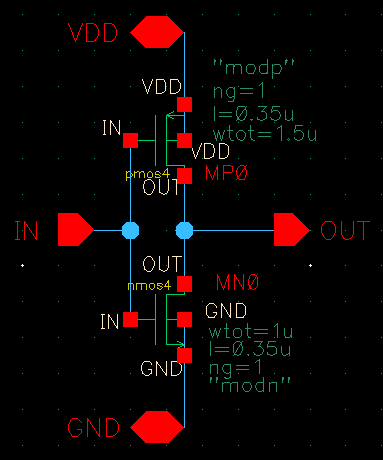
\includegraphics[scale=0.8]{images/esquematico1.png}
    \label{fig:esquematico1}
\end{figure}

\begin{figure}[htbp]
    \centering
    \caption{Leiaute da Implementação 1}
    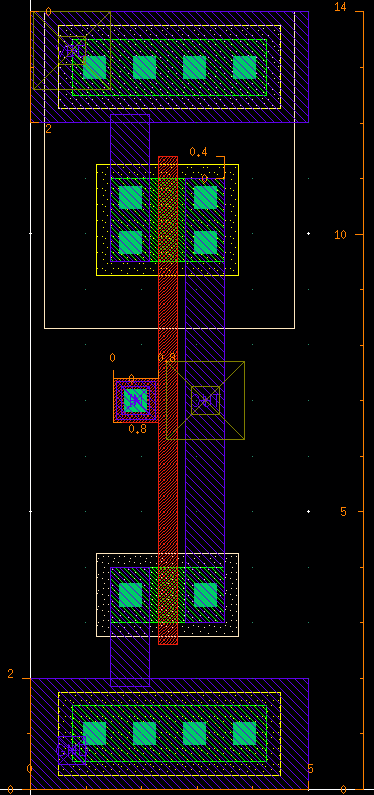
\includegraphics[scale=0.8]{images/layout1.png}
    \label{fig:leiaute1}
\end{figure}

\FloatBarrier

A Figura \ref{fig:LVS1} mostra o resultado da verificação \textit{Layout Versus Schematic} do leiaute da Figura \ref{fig:leiaute1}. Embora citadas agora, figuras de resultados de etapas de verificação não estarão presentes nas próximas seções por motivos de clareza do documento.

\begin{figure}[htbp]
    \centering
    \caption{LVS da implementação 1}
    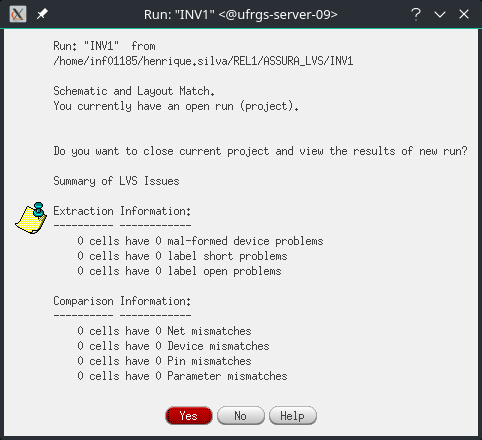
\includegraphics[scale=0.8]{images/LVS_2.png}
    \label{fig:LVS1}
\end{figure}

\FloatBarrier

\subsection{Implementação 2}\label{impl2}
A Implementação 2 possui transistores PMOS e NMOS ambos dimensionados em \SI{1.0}{\um} , sendo que tem em comum com a \nameref{impl1} quaisquer outras características aqui não mencionadas.\

A Figura \ref{fig:esquematico2} mostra o esquemático da porta lógica na ferramenta \virtuoso, e a Figura \ref{fig:leiaute2} mostra o seu respectivo leiaute. O leiaute foi feito de maneira semi-automática, utilizando as ferramentas de automação do \virtuoso.

\begin{figure}[htbp]
    \centering
    \caption{Esquemático da Implementação 2}
    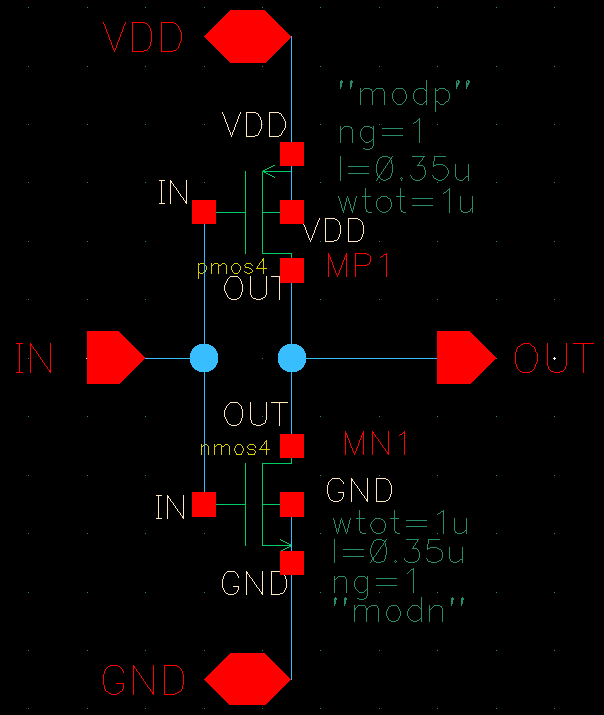
\includegraphics[scale=0.8]{images/esquematico2.png}
    \label{fig:esquematico2}
\end{figure}

\begin{figure}[htbp]
    \centering
    \caption{Leiaute da Implementação 2}
    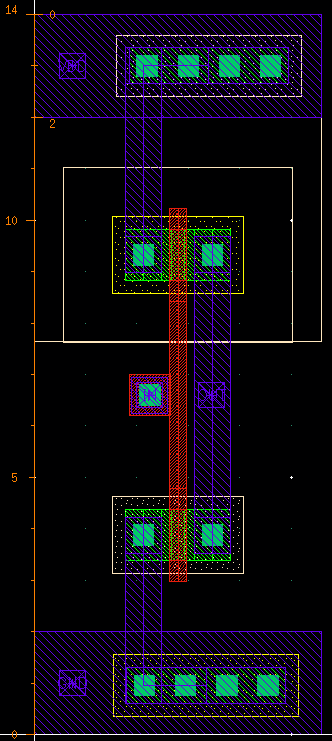
\includegraphics[scale=0.8]{images/layout2.png}
    \label{fig:leiaute2}
\end{figure}

\FloatBarrier

\subsection{Implementação 3}\label{impl3}
A Implementação 3 possui transistores PMOS e NMOS dimensionados respectivamente em \SI{10.5}{\um} e \SI{7.0}{\um}, sendo que tem em comum com a \nameref{impl1} quaisquer outras características aqui não mencionadas.\

A Figura \ref{fig:esquematico3} mostra o esquemático da porta lógica na ferramenta \virtuoso, e a Figura \ref{fig:leiaute3} mostra o seu respectivo leiaute. O leiaute foi feito de maneira semi-automática, utilizando as ferramentas de automação do \virtuoso.

\begin{figure}[htbp]
    \centering
    \caption{Esquemático da Implementação 3}
    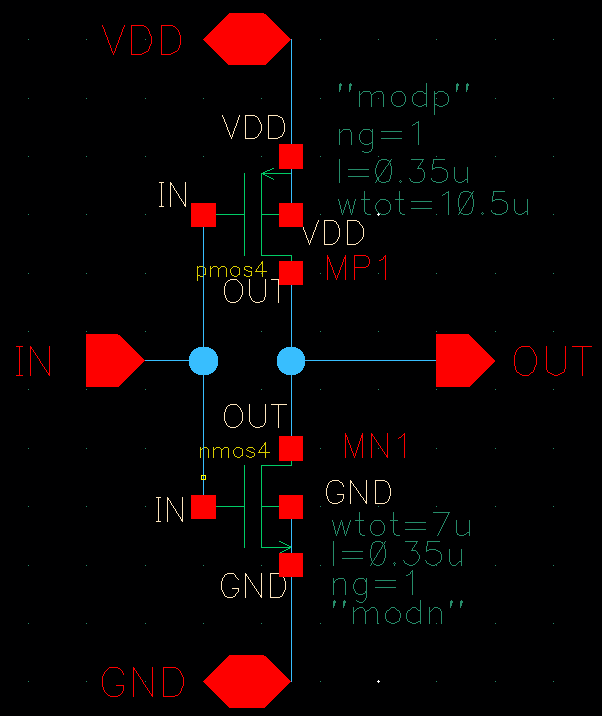
\includegraphics[scale=0.8]{images/esquematico3.png}
    \label{fig:esquematico3}
\end{figure}

\begin{figure}[htbp]
    \centering
    \caption{Leiaute da Implementação 3}
    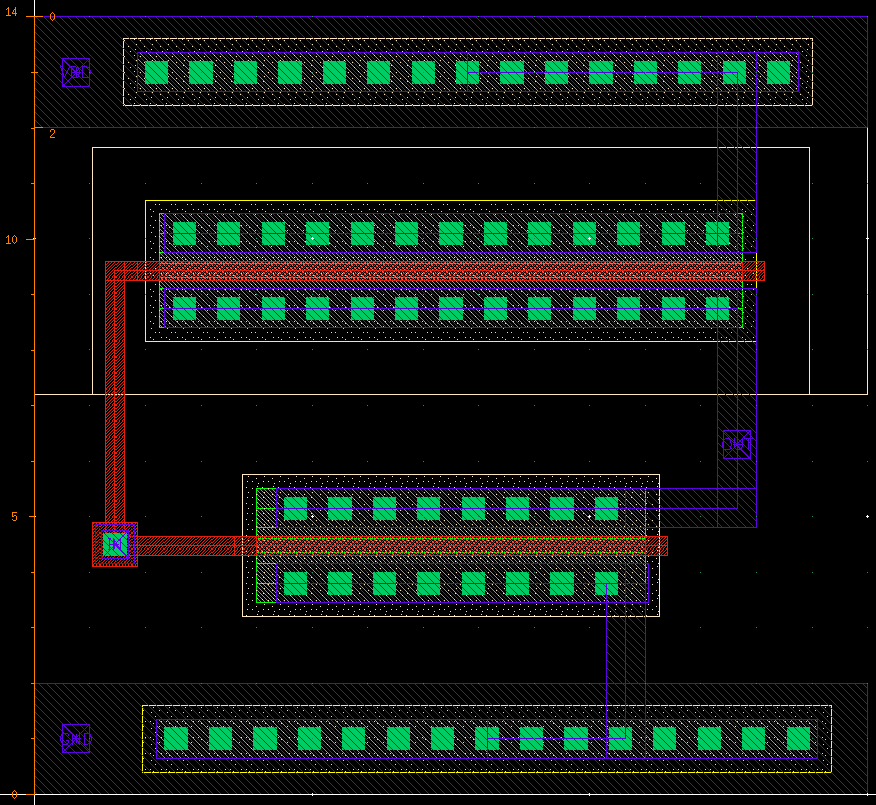
\includegraphics[scale=0.7]{images/layout3.png}
    \label{fig:leiaute3}
\end{figure}

\FloatBarrier

\subsection{Implementação 4}\label{impl4}
A Implementação 4 possui transistores PMOS e NMOS dimensionados respectivamente em \SI{7.0}{\um} e \SI{10.5}{\um}, sendo que tem em comum com a \nameref{impl1} quaisquer outras características aqui não mencionadas.\

A Figura \ref{fig:esquematico4} mostra o esquemático da porta lógica na ferramenta \virtuoso, e a Figura \ref{fig:leiaute4} mostra o seu respectivo leiaute. O leiaute foi feito de maneira semi-automática, utilizando as ferramentas de automação do \virtuoso.

\begin{figure}[htbp]
    \centering
    \caption{Esquemático da Implementação 4}
    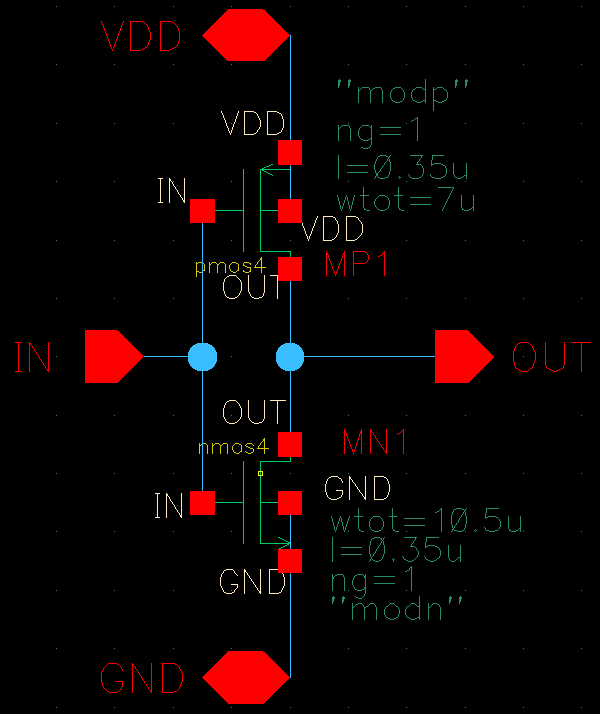
\includegraphics[scale=0.8]{images/esquematico4.png}
    \label{fig:esquematico4}
\end{figure}

\begin{figure}[htbp]
    \centering
    \caption{Leiaute da Implementação 4}
    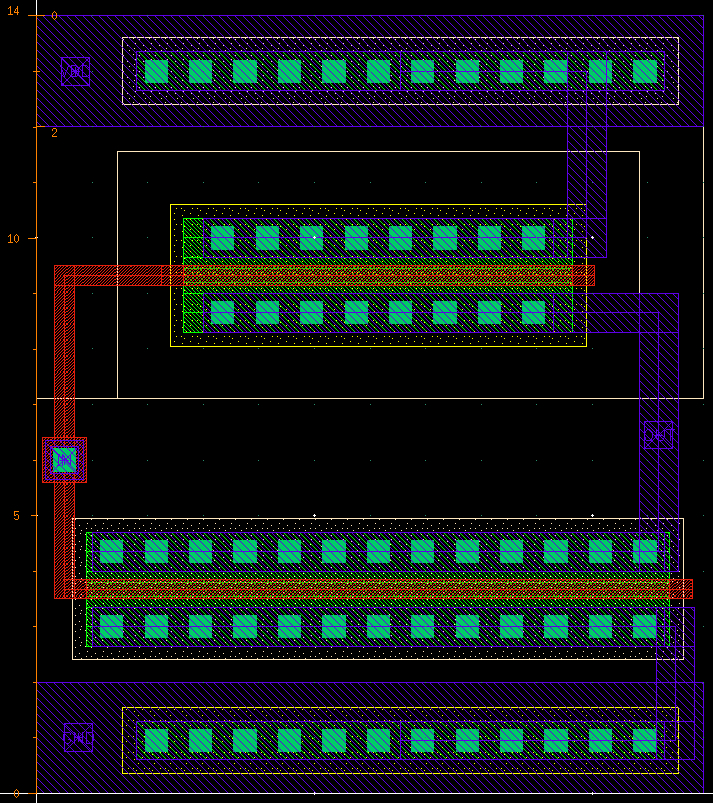
\includegraphics[scale=0.8]{images/layout4.png}
    \label{fig:leiaute4}
\end{figure}

\FloatBarrier

\section{Circuito}
O circuito para testes, representado na Figura \ref{fig:circuito}, consiste de 3 inversores em série, sendo que o primeiro e o último possuem dimensões W\textsubscript{p} e W\textsubscript{n} iguais. Além disso, podemos observar um sinal de entrada representado por uma fonte variável em pulsos na entrada e um capacitor polar de \SI{50.0}{\fF} após a saída do último inversor.\

Usaremos para a análise do circuito a entrada e a saída do segundo inversor\footnote{que será alterado em cada versão do circuito.}. Todas as simulações foram feitas utilizando a visão \textit{av\_extracted}\footnote{obtidas pela extração das capacitâncias parasitas de cada implementação.} dos inversores e definindo \SI{20}{\ns} como duração da simulação.

\subsection{Cadeia 1}
A Cadeia 1 de inversores utiliza a \nameref{impl1} como a implementação do segundo inversor. Os resultados da análise transiente desse circuito está no Capítulo \ref{resultados}.\

A Figura \ref{fig:circ_e1} mostra o esquemático do circuito na ferramenta \virtuoso, e a Figura \ref{fig:wave1} mostra o \textit{waveform} da simulação transiente do circuito.\

\begin{figure}[htbp]
    \centering
    \caption{Esquemático da Cadeia 1}
    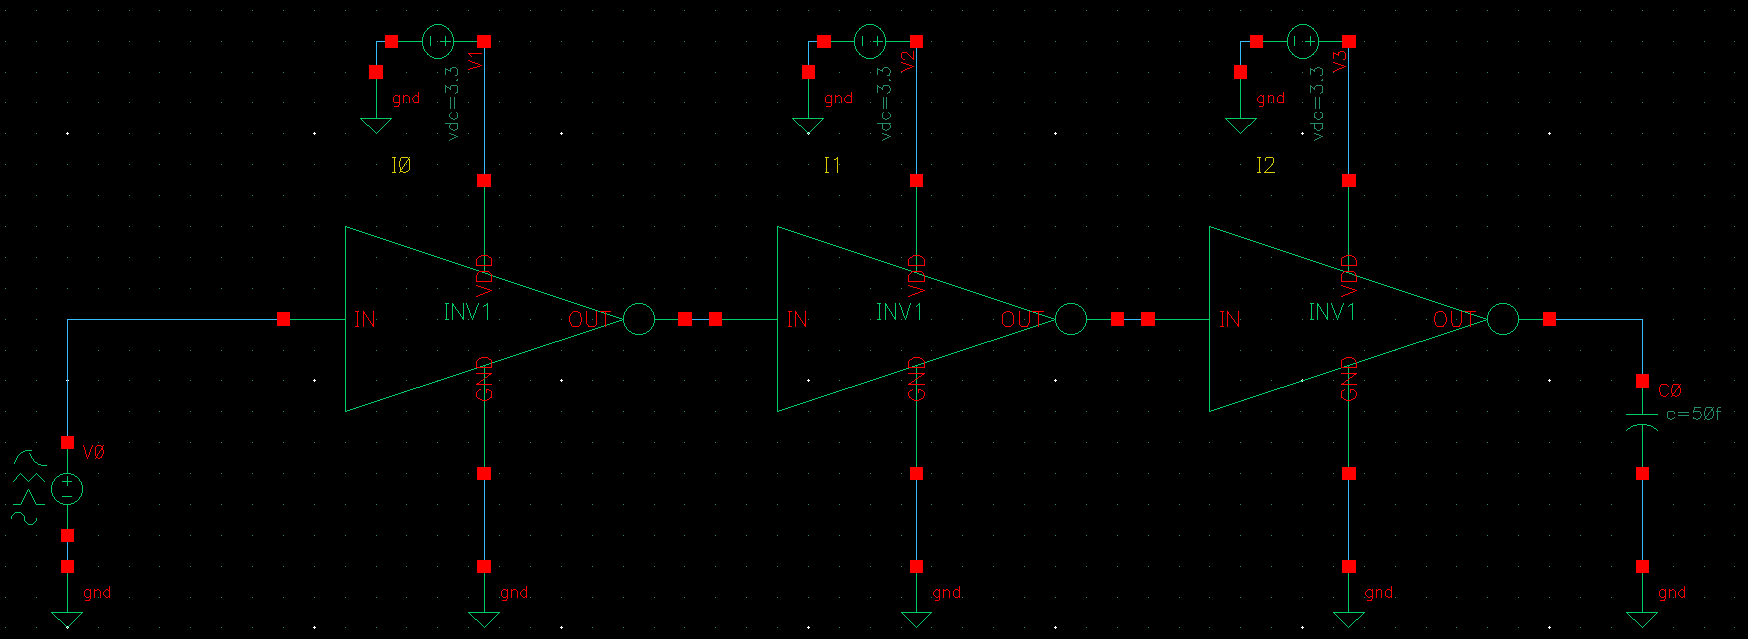
\includegraphics[scale=0.33]{images/circ1.png}
    \label{fig:circ_e1}
\end{figure}

\begin{figure}[htbp]
    \centering
    \caption{Waveform da simulação transiente da Cadeia 1}
    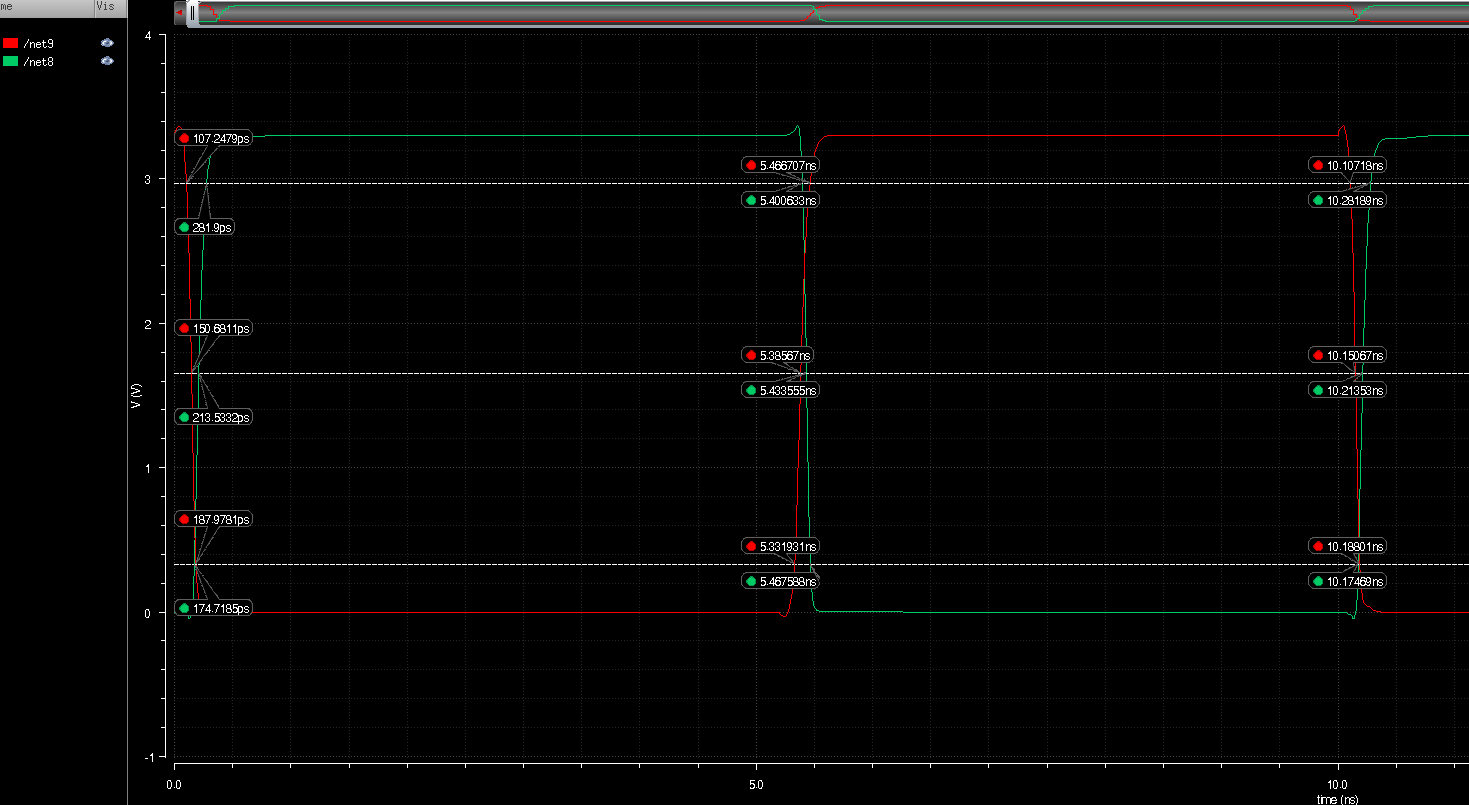
\includegraphics[scale=0.4]{images/wave_ex1.png}
    \label{fig:wave1}
\end{figure}

\FloatBarrier

\subsection{Cadeia 2}
A Cadeia 2 de inversores utiliza a \nameref{impl2} como a implementação do segundo inversor. Os resultados da análise transiente desse circuito está no Capítulo \ref{resultados}.\

A Figura \ref{fig:circ_e2} mostra o esquemático do circuito na ferramenta \virtuoso, e a Figura \ref{fig:wave2} mostra o \textit{waveform} da simulação transiente do circuito.\

\begin{figure}[htbp]
    \centering
    \caption{Esquemático da Cadeia 2}
    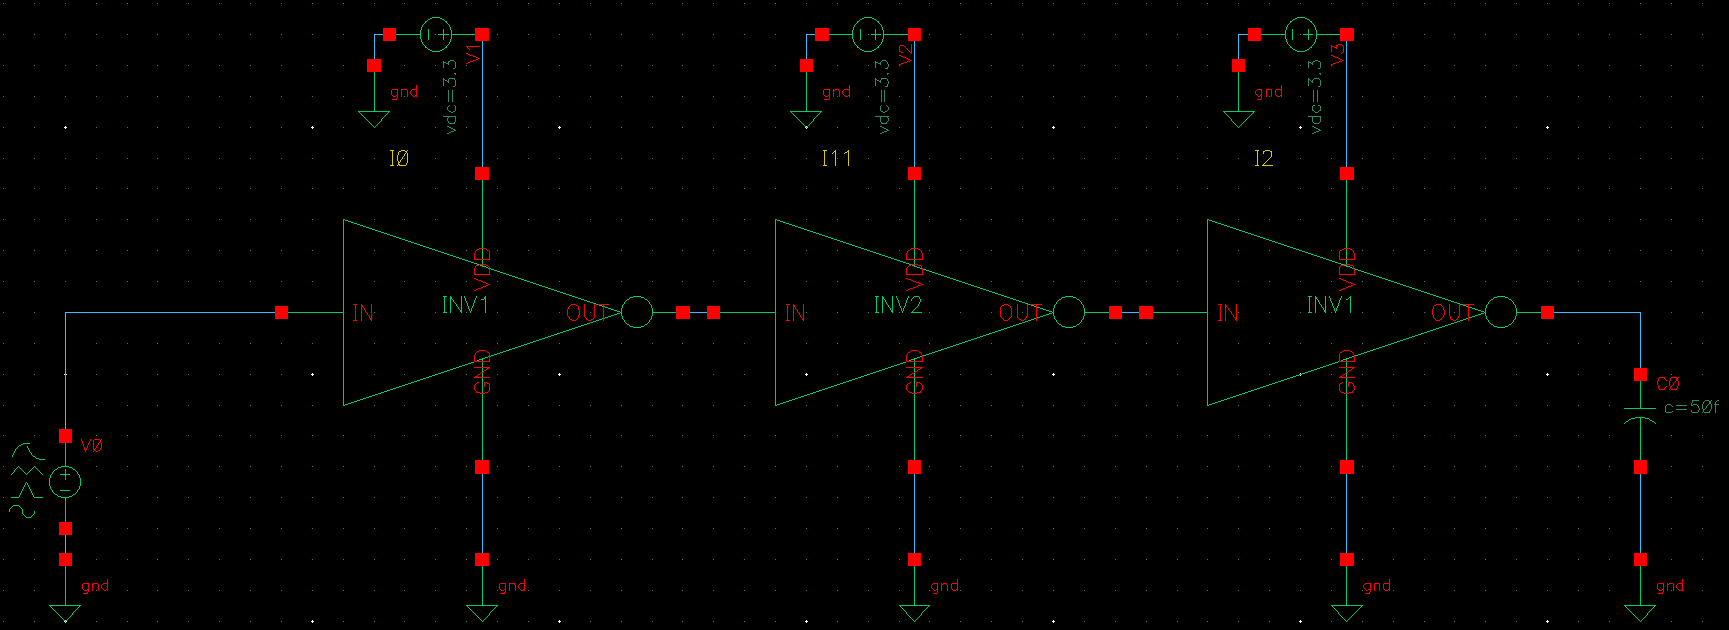
\includegraphics[scale=0.33]{images/circ2.png}
    \label{fig:circ_e2}
\end{figure}

\begin{figure}[htbp]
    \centering
    \caption{Waveform da simulação transiente da Cadeia 2}
    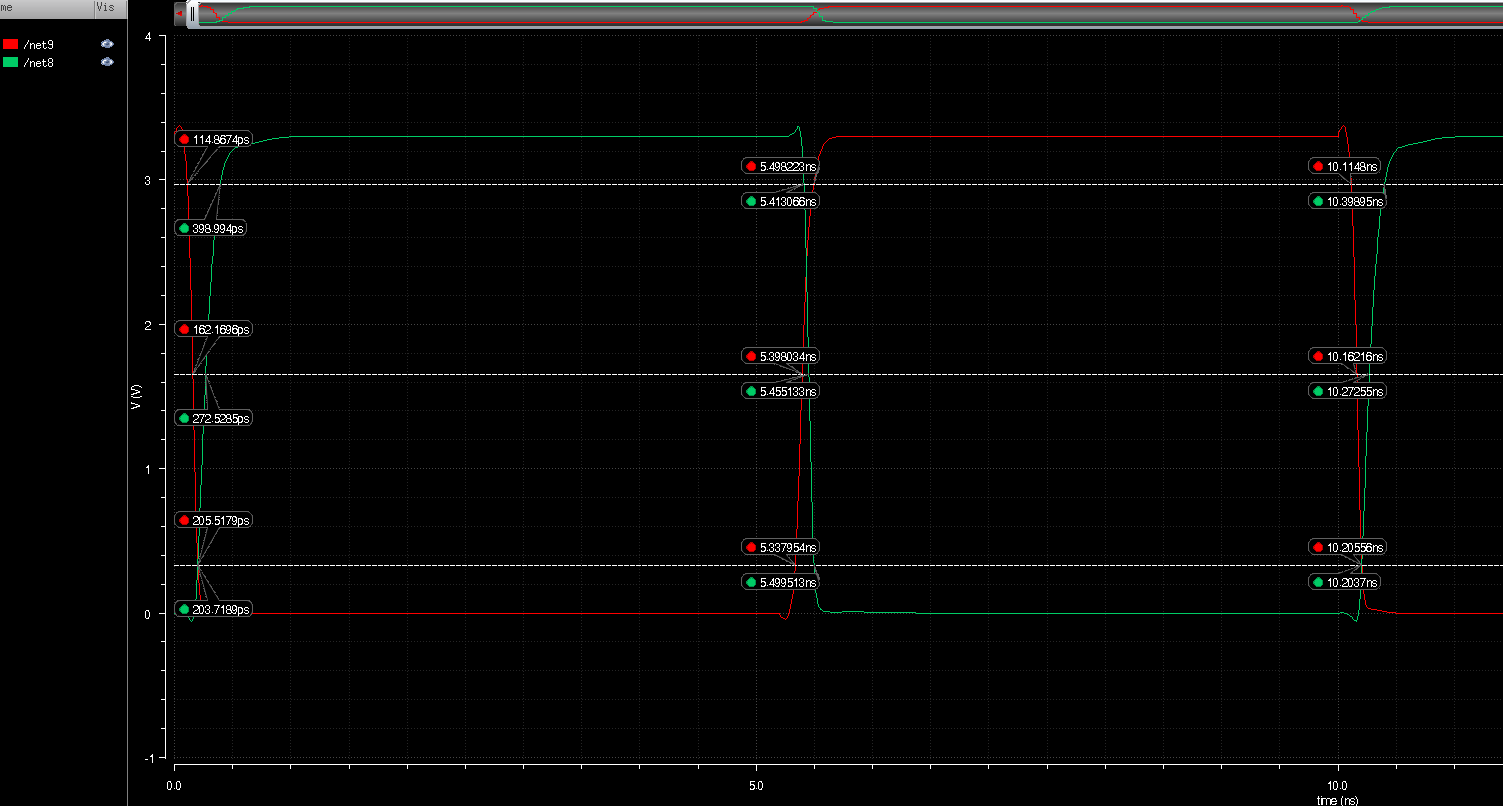
\includegraphics[scale=0.4]{images/wave_ex2.png}
    \label{fig:wave2}
\end{figure}

\FloatBarrier

\subsection{Cadeia 3}
A Cadeia 3 de inversores utiliza a \nameref{impl3} como a implementação do segundo inversor. Os resultados da análise transiente desse circuito está no Capítulo \ref{resultados}.\

A Figura \ref{fig:circ_e3} mostra o esquemático do circuito na ferramenta \virtuoso, e a Figura \ref{fig:wave3} mostra o \textit{waveform} da simulação transiente do circuito.\

\begin{figure}[htbp]
    \centering
    \caption{Esquemático da Cadeia 3}
    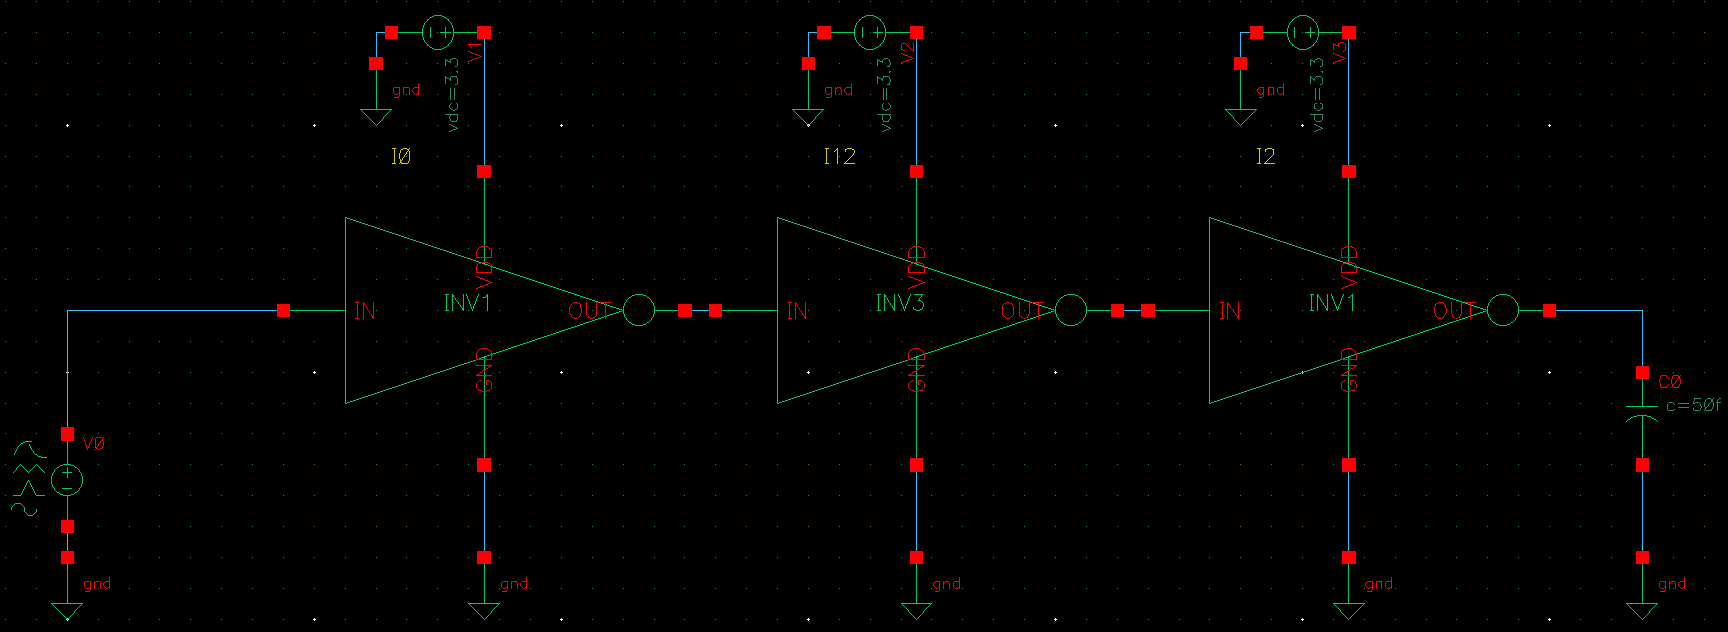
\includegraphics[scale=0.33]{images/circ3.png}
    \label{fig:circ_e3}
\end{figure}

\begin{figure}[htbp]
    \centering
    \caption{Waveform da simulação transiente da Cadeia 3}
    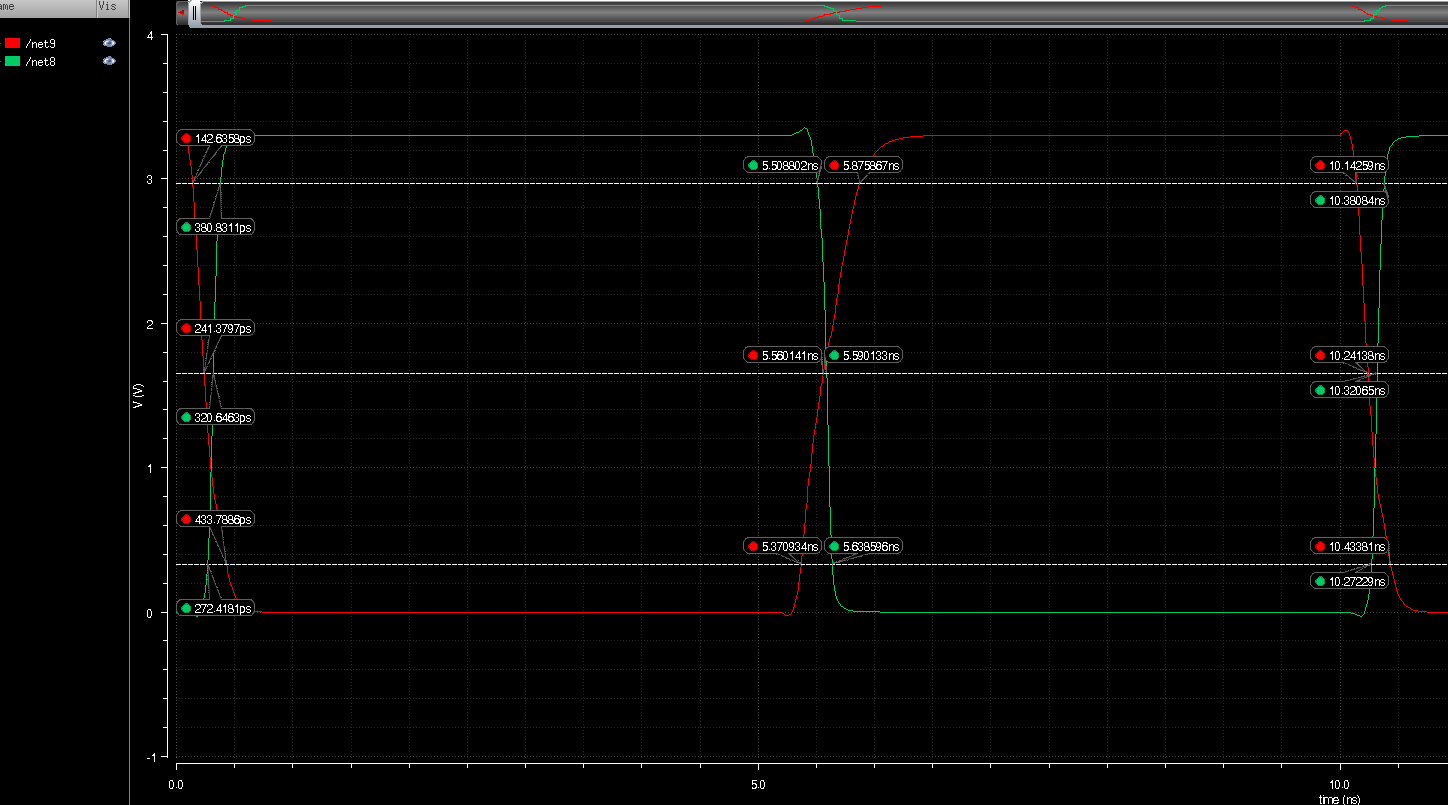
\includegraphics[scale=0.4]{images/wave_ex3.png}
    \label{fig:wave3}
\end{figure}

\FloatBarrier

\subsection{Cadeia 4}
A Cadeia 4 de inversores utiliza a \nameref{impl4} como a implementação do segundo inversor. Os resultados da análise transiente desse circuito está no Capítulo \ref{resultados}.\

A Figura \ref{fig:circ_e4} mostra o esquemático do circuito na ferramenta \virtuoso, e a Figura \ref{fig:wave4} mostra o \textit{waveform} da simulação transiente do circuito.\

\begin{figure}[htbp]
    \centering
    \caption{Esquemático da Cadeia 4}
    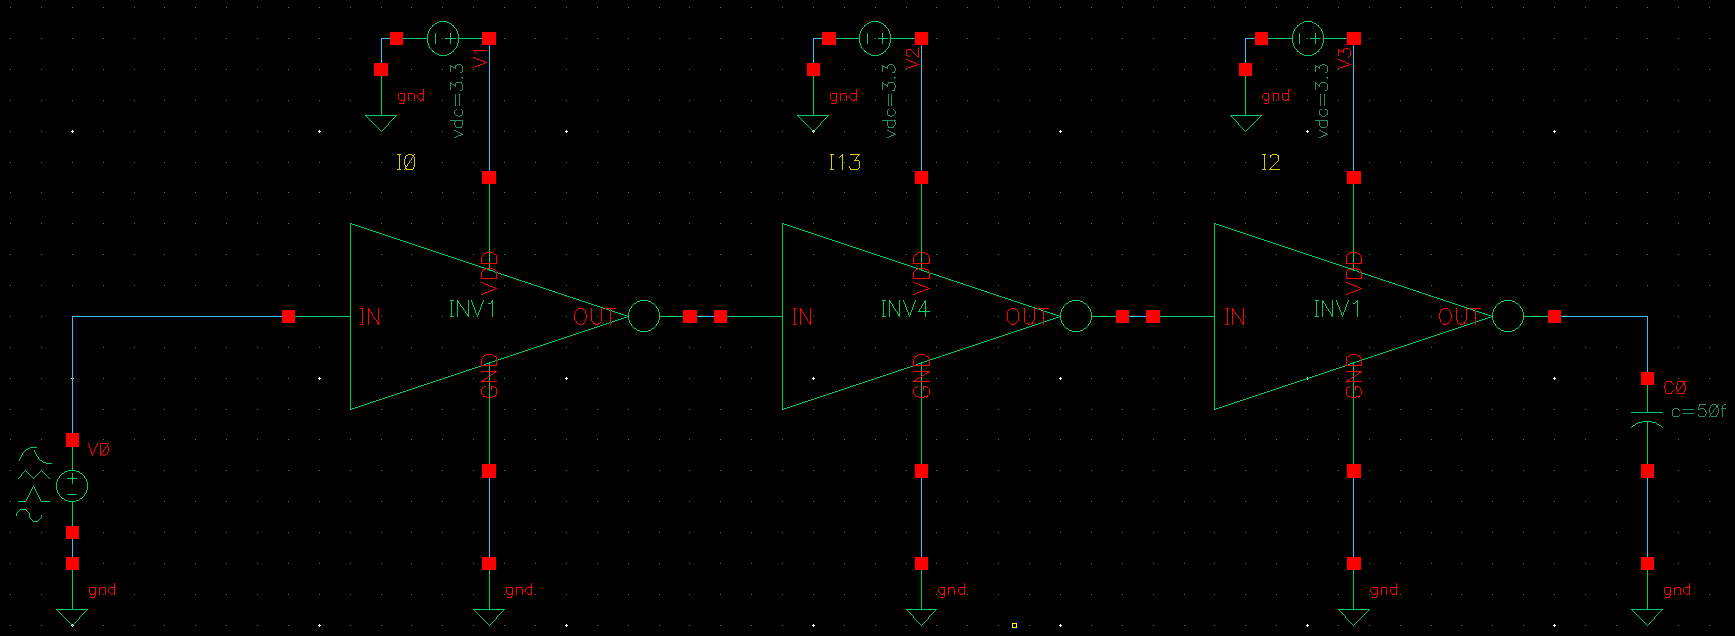
\includegraphics[scale=0.33]{images/circ4.png}
    \label{fig:circ_e4}
\end{figure}

\begin{figure}[htbp]
    \centering
    \caption{Waveform da simulação transiente da Cadeia 4}
    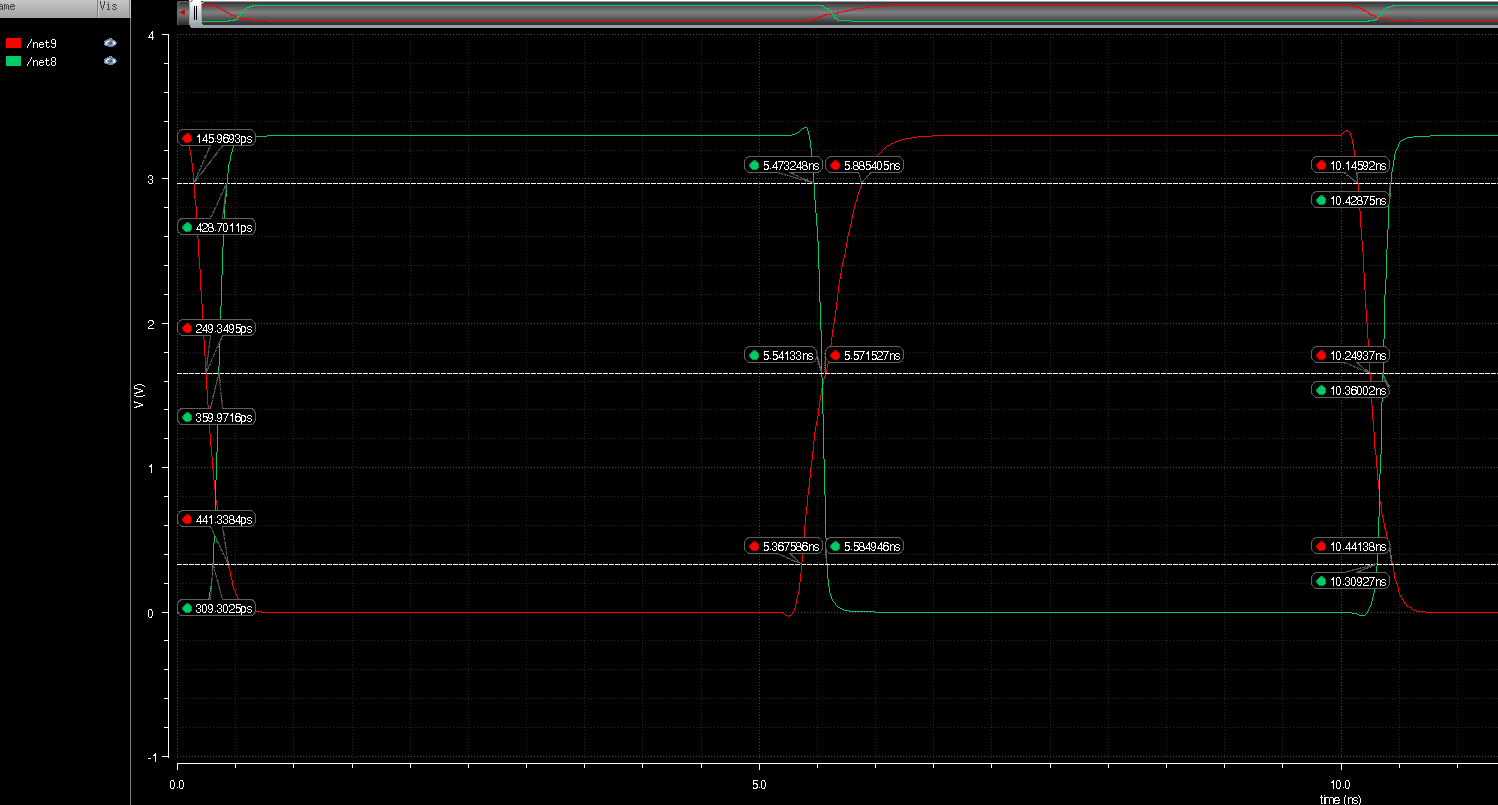
\includegraphics[scale=0.4]{images/wave_ex4.png}
    \label{fig:wave4}
\end{figure}

\FloatBarrier

\chapter{Resultados}\label{resultados}
Neste capítulo abordaremos os resultados obtidos nas simulações e discutiremos possíveis causas e consequências das escolhas de dimensionamento de cada inversor.

\section{Tabela}\label{tabela}
A Tabela \ref{tab:tempo} define os valores encontrados para cada uma das métricas temporais definidas no Capítulo \nameref{intro} para cada cadeia de inversores testada, e a Tabela \ref{tab:potencia} define as métricas de energia para as mesmas ditas cadeias.

% \begin{table}[ht]
%     \centering
%     \caption{Resultados temporais das simulações.}
%     \small
%     \label{tab:valores}
%     \sisetup{scientific-notation = true, round-mode = places, round-precision = 3}
%     \begin{tabular}{l l l l l}
%         \hline
%         Métrica
%         & Cadeia 1 & Cadeia 2 & Cadeia 3 & Cadeia 4 \\ \hline\hline
%         Tp\textsubscript{HL}
%         & \SI{0.047885}{\ns}    & \SI{0.057099}{\ns}    & \SI{0.029992}{\ns}    & \SI{0.030197}{\ns}    \\
%         Tp\textsubscript{LH}
%         & \SI{0.06286}{\ns}     & \SI{0.11039}{\ns}     & \SI{0.07927}{\ns}     & \SI{0.11065}{\ns}     \\
%         Tp\textsubscript{médio}
%         & \SI{0.0553725}{\ns}   & \SI{0.0837445}{\ns}   & \SI{0.054631}{\ns}    & \SI{0.0704235}{\ns}   \\
%         T\textsubscript{LH}
%         & \SI{0.1072}{\ns}      & \SI{0.19525}{\ns}     & \SI{0.10855}{\ns}     & \SI{0.11948}{\ns}     \\
%         T\textsubscript{HL}
%         & \SI{0.066955}{\ns}    & \SI{0.086447}{\ns}    & \SI{0.129788}{\ns}    & \SI{0.111712}{\ns}    \\
%         P\textsubscript{média}
%         & \SI{9.57e-6}{\W}      & \SI{11.85e-6}{\W}     & \SI{73.66e-6}{\W}     & \SI{68.89e-6}{\W}     \\
%         P\textsubscript{RMS}
%         & \SI{68.14e-6}{\W}     & \SI{62.22e-6}{\W}     & \SI{381.5e-6}{\W}     & \SI{343.2e-6}{\W}     \\
%         \hline
%     \end{tabular}
% \end{table}

\begin{table}[ht]
    \centering
    \caption{Resultados temporais das simulações.}
    \small
    \label{tab:tempo}
    \sisetup{scientific-notation = true, round-mode = places, round-precision = 3}
    \begin{tabular}{l l l l l l}
        \hline
        Cadeia
        & Tp\textsubscript{HL}
        & Tp\textsubscript{LH}
        & Tp\textsubscript{médio}
        & T\textsubscript{LH}
        & T\textsubscript{HL} \\ \hline
        \# 1
        & \SI{0.047885}{\ns} & \SI{0.06286}{\ns} & \SI{0.0553725}{\ns} & \SI{0.1072}{\ns}
        & \SI{0.066955}{\ns} \\
        \# 2
        & \SI{0.057099}{\ns} & \SI{0.11039}{\ns} & \SI{0.0837445}{\ns} & \SI{0.19525}{\ns}
        & \SI{0.086447}{\ns} \\
        \# 3
        & \SI{0.029992}{\ns} & \SI{0.07927}{\ns} & \SI{0.054631}{\ns} & \SI{0.10855}{\ns}
        & \SI{0.129788}{\ns} \\
        \# 4
        & \SI{0.030197}{\ns} & \SI{0.11065}{\ns} & \SI{0.0704235}{\ns} & \SI{0.11948}{\ns}
        & \SI{0.111712}{\ns} \\
        \hline
    \end{tabular}
\end{table}

\begin{table}[ht]
    \centering
    \caption{Resultados de consumo de potência.}
    \small
    \label{tab:potencia}
    \sisetup{scientific-notation = true, round-mode = places, round-precision = 3}
    \begin{tabular}{l l l}
        \hline
        $\cdots$
        & P\textsubscript{média}
        & P\textsubscript{RMS} \\ \hline
        \# 1
        & \SI{9.57e-6}{\W}  & \SI{68.14e-6}{\W} \\
        \# 2
        & \SI{11.85e-6}{\W} & \SI{62.22e-6}{\W} \\
        \# 3
        & \SI{73.66e-6}{\W} & \SI{381.5e-6}{\W} \\
        \# 4
        & \SI{68.89e-6}{\W} & \SI{343.2e-6}{\W} \\
        \hline
    \end{tabular}
\end{table}

\section{Discussão}\label{discussao}
Como análise retrospectiva, discutiremos os motivos de alguns dos resultados observados na Seção \ref{tabela}.

\subsection{Tempo de propagação}\label{tprop}
Como foi possível observar nos resultados das análises transiente dos diferentes dimensionamentos dos transistores NMOS e PMOS, pudemos notar que o tempo de propagação é inversamente proporcional à largura dos transistores.

A afirmação anterior, embora correta, esconde parte dos fatores em jogo ao redimensionar a largura de um transistor. Por exemplo, ao aumentar a largura do transistor PMOS a fim de contabilizar a lentidão do deslocamento de lacunas em relação ao deslocamento de eletrons, estamos, na verdade, diminuindo a resistência do transistor PMOS. Porém, ao fazer isso, também estamos aumentando de maneira diretamente proporcional a capacitância C\textsubscript{L} equivalente do circuito\footnote{causada pelo aumento físico das estruturas de difusão.}, o que afeta negativamente o tempo de propagação \cite{Rabaey1996Circuits}. Como nosso objetivo é diminuir o tempo de propagação, temos que encontrar uma relação ideal entre a resistência do transistor e a capacitância do circuito.

\subsection{Transições da Implementação 2}\label{timpl2}
Pela análise dos resultados obtidos para a segunda versão do circuito, que utiliza a \nameref{impl2}, foi possível observar que a transição mais rápida foi a de descida, ou seja, T\textsubscript{HL}.

Isso é consequência da característica elétrica inerente à transistores PMOS, que já foi citada brevemente na Seção \nameref{tprop}, que é o fato de lacunas se deslocarem mais lentamente que elétrons. Podemos mitigar essa dessincronia redimensionando o transistor PMOS para que esse seja cerca de 3 vezes maior que o NMOS.

\subsection{Dimensionamento e potência}\label{dimpot}
Também durante a análise dos resultados obtidos, foi possível observar que a potência nas versões do circuito que utilizavam as Implementações 3 e 4 cresceu uma ordem de magnetude em relação às versões que utilizavam Implementações menores.

Isso se deve ao mesmo fato discutido na Seção \nameref{tprop}, que é a relação entre dimensionamento de um transistor e sua resistência. Ao aumentar o dimensionamento, a resistência do transistor diminui e, por consequência, a corrente que passa pelo transistor aumenta. Com mais corrente passando pelo transistor numa mesma diferença de potêncial, temos $P = V*I$, e, assim, maior dissipação de potência pelo transistor.

Além disso, temos que o aumento dos transistores NMOS ou PMOS aumentam, por consequência, a capacitância de saída do inversor (representada na Figura \ref{fig:inversor} por C\textsubscript{L}\footnote{lembrando que esta é uma almálgama de todas as capacitâncias presentes na porta.}). Este aumento da capacitância leva a um aumento direto da energia tomada de V\textsubscript{DD} para carregar C\textsubscript{L}, onde, então, é dissipada ou guardada. A energia guardada é mais tarde dissipada no transistor NMOS durante a transição \textit{high-low}.

\subsection{Componentes do consumo de potência}\label{comppot}
Temos, como componentes do consumo de potência numa tecnologia CMOS, os seguintes itens:

\begin{itemize}[noitemsep]
    \setlength{\itemindent}{1em}
    \item \textbf{Resistências parasitas}: resistências não projetadas na fonte e no dreno causadas pela distância até a grade;
    \item \textbf{Dissipação dinâmica na capacitância de saída}: nas transições \textit{high-low} e \textit{low-high}, o capacitor ou é carregado pela rede \textit{pull-up} (dissipando e guardando energia) ou descarrega sua energia armazenada na rede \textit{pull-down}, definindo, assim, um gasto de energia de $C_L*V_{DD}^2$ por ciclo de transição;
    \item \textbf{Latchup}: transistores parasitas causados pelas diferentes difusões num circuito;
    \item \textbf{Consumo estático}: em temperaturas altas ($\approx$\SI{85}{\degreeCelsius}), o efeito de vazamento de \textit{junction currents} deixa de ser desprezível, aumentando por um fator 60 em relação à vazamentos em temperaturas ambiente normais;
    \item \textbf{Curto circuito em transientes}: em condições de transiente\footnote{ou seja, durante o switch de um transistor.}, existe um pico de corrente de curto circuito, dissipando, assim, energia não desprezível;
\end{itemize}

%%%%%%%%%%%%%%%%%%%%%%%%%%%%%%%%%%%%%%%%%%%%%%%%%%%%%%%%%%%%%%

\bibliographystyle{abntex2-alf}
\bibliography{biblio} 

\end{document}
